\chapter{Naturally Parameterized NLP framework}\label{CH4}

%%%%%%%%%%%%%%%%%%% SECTION 1 %%%%%%%%%%%%%%%%%%%%%%%%%%%%%
\section{Introduction}\label{CH4S1}
%%%%%%%%%%%%%%%%%%%%%%%%%%%%%%%%%%%%%%%%%%%%%%%%%%%%%%%%%%%
This chapter presents a parametric nonlinear programming (\acrshort{pnlp}) 
framework
that extends the problem solving capabilites of the Hybrid \acrshort{nlp} beam 
element beyond analyses concerned with mechanical loading. Such cases can be 
contact problems or structural sensitivity analysis. A strong feature of this 
framework lies in the utlizitation of homotopy continuation principles
in order to establish conditions of global
convergence to at least one solution. With the term ``solution" we broadly 
refer to any critical point for the objective function, which in the present 
context is the \acrshort{tpe}, with respect to the system variables. 

Homotopy continuation, which forms the backbone of the PNLP framework, has been 
the subject of extensive studies in the field of applied 
mathematics\cite{Allgower:2003,Rheinboldt:2000,Keller:1978,Li:1980,Chow:1978,Chow:1979,
Watson:1989,Watson:1990,Allgower:1981,Rheinboldt:1980,Rheinboldt:1983,Wayburn:1987}
as a technique for ``globalizing" root finding 
algorithms. That is, even if the initial guess is not in the neighborhood of a 
root, homotopy theory guarantees convergence to at least one root, given 
certain regularity conditions hold. These conditions in essence establish the 
existence of a smooth path connecting the initial guess and that root.  When 
applied to finding a root of a system of equations $F(x)=0$, this can be done 
by introducing an ``easy" problem whose a solution is easy to find, say 
$x-x_0=0$, and then construct a homotopy function $H(x,t) = 
tF(x)+(1-t)(x-x_0)$, 
which represents a system of $n$ equations with $n+1$ unknowns. The system  
$H(x,t)=0$ is sequantially solved for a discretization of $t\in[0,1]$, starting 
at $t_0=0$, where the solution is known (``initial guess"). When $t=1$ we have 
arrived at a root of the initial problem $F(x)=0$. The process of varying $t$ 
from 0 to 1 and solving the homotopy function is called deformation (not to be 
confused with mechanical deformation) and construction of such a homotopy 
function is called artificial homotopy.  It is clear that the same principles 
can be applied if system $F(x)=0$ is undetermined, with $n$ equations, $n+1$ 
unknowns and a solution is available or can be found easily. In a nonlinear 
optimization context, application of the same principles have led to the 
formulation of global optimization 
algorithms\cite{Kojima:1984,Gfrerer:1985,Guddat:1990,Gfrerer:1983,Zangwill:1981,Poore:1990,
Jongen:1990,Tiahrt:1989}. In addition, this 
framework highlights the firm theoretical
underpinnings of various incremental methods that
have been developed independently over the past decades for the numerical 
treatment 
of engineering 
problems\cite{Crisfield3,Wempner:1971,Bergan:1978,Bergan:1978b,Batoz:1979,Riks:1979,
Ramm:1981,Watson:1985,Sideris:2017,Byrne:1985,Ushida:1984,Borkovsky:2010,Besanko:2010,
Herings:2010,Bartovn:2016,Barendrecht:2018}. Application of this framework for 
approximating roots 
of systems of equations is commonly referred to as numerical continuation, 
whereas in the context of finding and characterizing optimizers, it is termed 
parametric 
optimization or \acrshort{pnlp}.
  
In structural mechanics, differential equilibrium equations can be reformulated 
as an optimization problem due to the existence of a variational structure, as 
discussed in Chapter \ref{chapter:CH2}. Thus, the \acrshort{pnlp} framework 
provides a suitable and versatile engine for generating global solutions to 
engineering problems using the Hybrid 
\acrshort{nlp}-based element, since it allows for the incorporation of 
constraint
specifications directly at the minimization statement. It is shown that, in the 
presence of inequality constraints, the global path that connects the initial 
guess to a critical point is continuous but piecewise 
differentiable\cite{Kojima:1984,Guddat:1990,Gfrerer:1985}. Finally, utilizing 
the underlying 
homotopy arguments, we establish the conditions under which the path we follow 
is unique and convergent to at least one critical point. Non-uniqueness of the 
homotopy path implies the existence of bifurcation points. Because the 
derivations do not make use of artificial functions in order to introduce 
initial guesses, we termed the formulation as Naturally Parameterized NLP 
(\acrshort{npnlp}). While this has the downside of requiring a known solution 
of the system in order to initiate the homotopy deformation process, in 
structural mechanics such states can often be found easily (e.g. initial 
configuration).

This chapter is divided into five sections. In the first section we give an 
overview of homotopy continuation as applied in (globally) solving systems of 
nonlinear equations and in parametric optimization. In the second section we
formulate the \acrshort{npnlp} framework for the hybrid element and in section 
three we outline the conditions that both the \acrshort{tpe} and the element 
constraints need to satisfy in order to guarantee global convergence following 
a unique path. A brief note on bifurcating paths is also included but the topic 
is not explored further herein. Finally, we demonstrate the capabilities of the 
framework through a set of problems from the 
mechanics and applied mathematics literature.

%%%%%%%%%%%%%%%%%%%%%%   SECTION 1  %%%%%%%%%%%%%%%%%%%%%%%%%%%%%%%%
\section{Homotopy Continuation}\label{CH4-S1}
%%%%%%%%%%%%%%%%%%%%%%%%%%%%%%%%%%%%%%%%%%%%%%%%%%%%%%%%%%%%%%%%%%%%

%%%%%%%%%%%%%%%%%%%%%%  SECTION 1 - SUBSECTION 1  %%%%%%%%%%%%%%%%%%
\subsection{Main Idea}\label{CH4-S1SS1}

The application of numerical approximation methods in virtually all engineering
and scientific problems leads, generally, to an algebraic system of equations,
$\bvec{F}$, to
be solved for the system unknowns, $\bvec{x}$. This system, of which we seek one
or more roots, is expressed in the following form:
\begin{equation}
\bvec{F}(\bvec{x})=\bvec{0}
\label{eq:P1}
\end{equation}
where for simplicity we assume that $\bvec{x}\in\mathbb{R}^n$ and
$\bvec{F}:\mathbb{R}^n\rightarrow\mathbb{R}^n$ is a
sufficiently smooth vector function. Given 
an initial estimate, $\bvec{x}_0$,
one can use the Newton method to iteratively find a root:
\begin{equation}
\bvec{x}_{i+1} = \bvec{x}_i-\bmat{F_x}^{-1}_{,i}\bvec{F}_i,\quad i=0,1,\cdots
\label{eq:NEWTON}
\end{equation}
This approach will yield a solution if i) $\bvec{x}_0$ is already in the 
vicinity
of a root and ii) if the Jacobian $\bmat{F_x}$ is not singular for any of 
the iterates$\{\bvec{x}\}_i$. The main idea of the homotopy continuation is to 
overcome the difficulty that
singularity points pose by imbedding problem (\ref{eq:P1}) in a higher
dimensional space where both $\bvec{x}$ and parameter $t$ are considered 
independent variables.
This is done by pairing function $\bvec{F}$ with a simpler problem,
$\bvec{G}:\mathbb{R}^n\rightarrow\mathbb{R}^n$ which has a trivial solution 
$\bvec{G}(\bvec{x}_0)=\bvec{0}$, using a homotopy function, 
$\bvec{H}(\bvec{x},t)$. 
For $\bvec{H}:\mathbb{R}^n\times\mathbb{R}\rightarrow \mathbb{R}^n$ we require
that
i) $\bvec{H}=\bvec{0}$ for all $(\bvec{x},t)$ and ii)
$\bvec{H}(\bvec{x}_0,0)=\bvec{G}(\bvec{x}_0)$ and
$\bvec{H}(\bvec{x}_1,1)=\bvec{F}(\bvec{x}_1)=\bvec{0}$. Under certain 
regularity 
conditions, the Jacobian of
$\bvec{H}$, $\bmat{DH}$, is of full rank even at points where $\bmat{F_x}$ 
is
singular and, by the implicit function theorem, there exists a unique 
differentiable path
$\mathit{\Gamma}:\mathbb{R}\rightarrow\mathbb{R}^{n}\times\mathbb{R}$, 
with $\mathit{\Gamma}(s)=(\bvec{x}(s),t(s))$, $s\in\mathbb{R}$ and
$\bvec{H}(\mathit{\Gamma})=\bvec{0}$.
This path connects the solution of the trivial problem, $\bvec{x}_0$, at $t_0=0$
with at least one root of $\bvec{F}$, $\bvec{x}_1$, when $t=1$ and can be
tracked using numerical continuation\cite{Allgower:2003}. The process of 
varying parameter $t$ from $0\rightarrow 1$
is referred to as deformation from the simple problem $\bvec{G}=\bvec{0}$ to 
the initial one, $\bvec{F}=\bvec{0}$, and such a path is depicted in Fig. 
\ref{fig:FIG29}.

\begin{figure}[t]
	\centering
	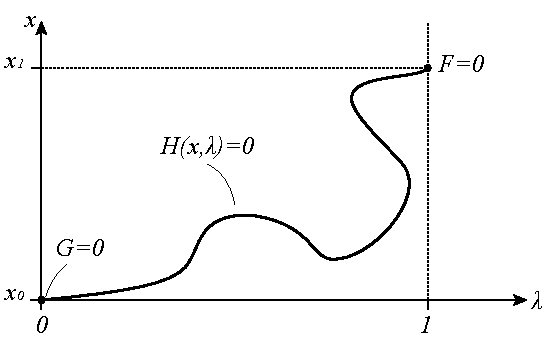
\includegraphics[scale=1.1]{FIG29.pdf}
	\caption{A homotopy path connecting the trivial solution of $G=0$ 
		to a root of $F=0$ for a single scalar equation dependent on $x$.}
	\label{fig:FIG29}
\end{figure}
The path $\mathit{\Gamma}$ depends on how $\bvec{H}$ is defined, which in turn 
is determined by the choice for $\bvec{G}$. We distinguish two general
cases of homotopy imbeddings: artificial and natural.

One typically resorts to artificial homotopies when a simple solution to problem
(\ref{eq:P1}) is generally not available. The homotopy parameter
$t$ and the simpler problem $\bvec{G}$ are then simply devices that
initialize the deformation process. In this
case, only the final point $(\bvec{x}_1,1)$ is of interest and not the path
$\mathit{\Gamma}$. A commonly used form
of artificial imbedding is the convex homotopy: 
\begin{equation}
	\bvec{H}(\bvec{x},t) = t\bvec{F}(\bvec{x})+(1-t)\bvec{G}(\bvec{x})=\bvec{0}
	\label{eq:homotopy1}
\end{equation}
Among the variety of convex homotopy functions that have been
developed, the ones most frequently used in implementations are:
\begin{itemize}
	\item{\makebox[5cm][l]{Probability-one homotopy:}
		$\bvec{G}(\bvec{x})=\bvec{x}-\bvec{x}_0$}
	\cite{Chow:1978,Watson:2002}
	\item{\makebox[5cm][l]{Newton homotopy:} $\bvec{G}(\bvec{x}) =
		\bvec{F}(\bvec{x})-\bvec{F}(\bvec{x}_0)$}
	\cite{Keller:1978,Smale:1976}
	\item{\makebox[5.01cm][l]{Affine homotopy:} $\bvec{G}(\bvec{x}) =
		\bmat{F_x}_0(\bvec{x}-\bvec{x}_0)$}\ \cite{Garcia:1980,Wayburn:1987}
\end{itemize}
On the other hand, systems whose response depends on
variations of a parameter, $t$, that has physical meaning can be recast as 
natural homotopies as follows:
\begin{gather}
	\bvec{R}(\bvec{x})=0 \xrightarrow{\text{parameterization}} 
	\bvec{R}(\bvec{x},t)=0
	\label{eq:Natural}
\end{gather}

Frequently, in such cases an initial state of the system, $\bvec{R}_0$, is
easily found and the deformation process starts from there. The
process ends when one or more target states are found, which, by convention, 
correspond to $t=1$. In constrast with artificial imbeddings, the path
$\mathit{\Gamma}$ generated by Eq. (\ref{eq:Natural}) is also of interest
because all $(\bvec{x},t)\in\mathit{\Gamma}$ represent states of the
system. As an example, the residual balance equations in nonlinear mechanics, 
$\bvec{R}(\bvec{u})=\bvec{0}$, can be cast as a natural homotopy,
$\bvec{R}(\bvec{u},t)=\bvec{0}$, where $\bvec{u}$ is the displacement vector 
and $t$ represents the load intensity of extern loads.

\begin{figure*}[h]
	\centering
	\subfloat[][]{{\includegraphics[width=7.0cm]{FIG30_POLYDEMO.pdf}}\label{fig:FIG30_1}}%
	\qquad
	\subfloat[][]{{\includegraphics[width=7.15cm]{FIG30_POLYDEMO2.pdf}}\label{fig:FIG30_2}}%
	\caption{Homotopy paths for \textbf{(a)} $f(x)=x^3-6x^2+21x-26=0$, with 
		starting point
		$x_0=0$ and convergence at root $x_1=2$ when $t=1$ and 
		\textbf{(b)}
		truss, with initial state the undeformed
		configuration($x_0=0$) and target load level $P=0.03$.}%
	\label{fig:FIG30}%
\end{figure*}
\clearpage
A simple demonstration is provided in Fig. \ref{fig:FIG30}, where the
three artificial homotopies
mentioned above are used in two problems. In the first problem
(Fig. \ref{fig:FIG30_1}), we find a root 
of a cubic polynomial, while in the second (Fig. \ref{fig:FIG30_2}) 
we solve the 
one degree of freedom truss for target state corresponding to load $P=0.03$. 
Details for this example are taken from \cite{Rheinboldt:1981}. We see
from the truss case that while, in principle, artificial imbeddings can be 
used for systems that can be naturally parameterized, the intermediate solution
points on the path do not correspond to actual equilibrium configurations. 

%%%%%%%%%%%%%%%%%%%%%%  SECTION 1 - SUBSECTION 2  %%%%%%%%%%%%%%%%%%
\subsection{Regularity and Existence of Homotopy Paths}\label{CH4-S1SS2}

From the discussion so far it is evident that the study of mappings
$\bvec{H}:\mathbb{R}^{n+1}\rightarrow\mathbb{R}^n$ is of primary importance. 
Consider such a mapping, $\bvec{H}(\bvec{v})$, which is at least 
of $C^k$ continuity, $k\geq 2$, with $\bvec{v}\in\mathbb{R}^{n+1}$ and $t$ 
being its $(n+1)$th component. 
For any given $\bvec{w}\in\mathbb{R}^n$, the equation 
$\bvec{H}(\bvec{v})=\bvec{w}$
represents a system of $n$ equations with $n+1$ unknowns and we designate the
subset of $\mathbb{R}^{n+1}$ satisfying this system as follows:
\begin{equation*}
	\bvec{H}^{-1}(\bvec{w}) = \{\bvec{v}\in\mathbb{R}^{n+1}\ |\ 
	\bvec{H}(\bvec{v})=\bvec{w}\}\subseteqq\mathbb{R}^{n+1}
\end{equation*}
\begin{definition}[Regular values of $\bvec{H}$]
	An element $\bvec{w}\in\mathbb{R}^n$ is a regular value of 
	$\bvec{H}:\mathbb{R}^{n+1}\rightarrow\mathbb{R}^n$ if its Jacobian,
	$\bmat{DH}$, has rank $n$ for all $\bvec{v}\in \bvec{H}^{-1}(\bvec{w})$.
	\label{def:reg}
\end{definition}
\begin{definition}[Regular points of $\bvec{H}$]
	An element $\bvec{v}\in\mathbb{R}^{n+1}$ is a regular point of
	$\bvec{H}:\mathbb{R}^{n+1}\rightarrow\mathbb{R}^n$ if its Jacobian at that 
	point is of rank $n$.
	\label{def:reqpoint}
\end{definition}
The components of the $n\times (n+1)$ Jacobian are given by $\bmat{DH}_{ij} = 
\partial H_i^{}/\partial v_j$. It follows that if $\bvec{w}$ is a regular value 
for $\bvec{H}$, then all $\bvec{v}\in\bvec{H}^{-1}(\bvec{w})$ are regular 
points. The following lemma\cite{Allgower:2003}, stated 
here without proof, plays a constitutive role in homotopy continuation theory:

\begin{lemma}
	Let $\bm{H}:\mathbb{R}^{n+1}\rightarrow\mathbb{R}^n$ be a $C^k$ map, $k\geq
	2$, and having $\bvec{0}$ as a regular value. Then, the set 
	$\bvec{H}^{-1}(\bvec{0})$ 
	is a $C^k$ 1-dimensional manifold in $\mathbb{R}^{n+1}$, comprised of
	non-intersecting components
	that are either i) homeomorphic with the unit circle $S^1$ (loops) or 
	ii) homeomorphic with the real line $\mathbb{R}$ (paths).
	\label{Lemma:manifold}
\end{lemma}
We refer to the collection of paths and loops in $\bvec{H}^{-1}(\bvec{0})$ as
(connected) components. Figure \ref{fig:FIG31} depicts a collection of such 
components for illustrative purposes. If $\bvec{0}$ is a regular value of 
$\bvec{H}$, by the
implicit function theorem, a path(loop) $\mathit{\Gamma}$ can be described as a
$C^k$ 
map $\mathit{\Gamma}:\mathbb{R}(\text{or}\ S^1)\rightarrow\mathbb{R}^{n+1}$ 
such that
$\bvec{v}=\bvec{v}(s)$. The tangent to that curve is given by
$\dot{\bvec{v}}=d\bvec{v}^{}/ds$ and is always a non-zero vector(cf.
\cite{Allgower:2003,Garcia:1980}).

\begin{figure}[t]
	
	\centering
	\includegraphics[scale=0.7]{FIG31_MAP.pdf}
	\caption{Components of $\bvec{H}^{-1}(\bvec{0})$ in $\mathbb{R}^{n+1}$.}
	\label{fig:FIG31}
\end{figure}

Consider now the case of $\bvec{H}(\bvec{v})$ where the $n+1$-th component of 
$\vec{v}$ can be regarded as a special parameter of 
interest, designated as $t$. We are interested in the zero points of 
$\bvec{H}$:
\begin{equation}
	\bvec{H}(\bvec{x},t)=0
	\label{eq:GENHOM}
\end{equation}
\noindent where $\bvec{x}\in\mathbb{R}^n$, 
$t\in\mathbb{R}$. Any given initial point $(\bvec{x}_0,0)$ that satisfies Eq.
(\ref{eq:GENHOM}) sets us on a component of $\bm{H}^{-1}(\bvec{0})$ which we 
will
designate as $\mathit{\Gamma}_0$ and define as follows:
\begin{equation}
	\mathit{\Gamma}_0=\{(\bvec{x},t)\ |\ 
	\bvec{x}\in\mathbb{R}^n,\ t\in\mathbb{R},\ (\bvec{x}_0,0)\ \text{in}\ 
	\Gamma_0,\ \bvec{H}(\bvec{x}_0,0)=\bvec{0}\}
	\label{eq:PATH}
\end{equation}
In most applications we want to ensure the initial point $\bvec{x}_0$ sets us 
on 
a component $\mathit{\Gamma}_0$ which is a path, not a loop. Under the 
smoothness and regularity assumptions, the condition which guarantees that is 
for
the $n\times n$ submatrix $\bmat{DH}=\partial \bvec{H}^{}/\partial \bvec{x}$ to 
be
non-singular at $\bvec{x}_0$\cite{Garcia:1980}. More conditions are generally
required to guarantee that the path will reach $t=1$ at least once and 
depend on the particular form of $\bvec{H}$. The interested reader can refer to
\cite{Allgower:2003}, which provide proofs of existence and convergence for
various types of homotopies. In addition, it is customary to formulate
homotopies with $t\in[0,1]$. In our formulation we adhere to the
convention that a solution is reached when $t=1$. However, as is the case 
in many 
practical applications, the restriction of $t$ to lie in the unit
interval is relaxed and the parameter is allowed to take values outside of that 
range. The expectation is that more solutions will be
reached by crossing the level $t=1$ multiple times. However, it should 
be noted that homotopy theory guarantees the (global) convergence 
to one solution $(\bvec{x}_1,1)$. While certain homotopy imbeddings can find 
multiple
solutions when tracking numerically a single component
path\cite{Keller:1978,Lin:1987,Sun:1995}, it is difficult to establish
conditions that guarantee convergence to many or all solutions in
general\cite{Sun:1995}. 

%%%%%%%%%%%%%%%%%%%%%%  SECTION 1 - SUBSECTION 3  %%%%%%%%%%%%%%%%%%
\subsection{Parametric Nonlinear Programming}\label{CH4-S1SS3}

Our derivations follow
closely the works of Kojima \& Hirabayashi\cite{Kojima:1984}, Gfrerer et
al.\cite{Gfrerer:1983}, Gfrerer, Wacker et al.\cite{Gfrerer:1985}, Guddat et
al.\cite{Guddat:1990}.
Consider the following one-parameter optimization program:
\begin{equation}
	\hspace*{-4.5cm}\textbf{P}(t): \hspace*{3.8cm}\text{min}\{f(\bvec{x},t)\ |\
	\bvec{x}\in\Omega(t),\
	t\in\mathbb{R}\}
	\label{eq:PNLP}
\end{equation}
\noindent with
\begin{equation}
	\Omega(t)=\{\bvec{x}\in\mathbb{R}^n\ |\ h_i(\bvec{x},t)=0,\ 
	i\in\mathit{I}_h,\
	g_j(\bvec{x},t)\leq 0,\ j\in\mathit{I}_g\}
	\label{eq:ConstraintSet}
\end{equation}
\noindent where we assume that functions
$f:\mathbb{R}^{n+1}\rightarrow\mathbb{R},h_i:\mathbb{R}^{n+1}\rightarrow\mathbb{R}$
and $g_j:\mathbb{R}^{n+1}\rightarrow\mathbb{R}$  are considered to
be $C^k$, $k\geq 3$, $\mathit{I}_h=\{1,\cdots,l\}$,
$\mathit{I}_g=\{1,\cdots,p\}$ and $l\ll n$, $p\ll n$. Let
$\mathcal{L}(\bvec{x},\bvec{\lambda},\bvec{\mu},t)$ be the corresponding 
Lagrangian 
function of
problem \textbf{P}$(t)$:
\begin{equation}
	\mathcal{L}(\bvec{x},\bvec{\lambda},\bvec{\mu},t) =
	f(\bvec{x},t)+\sum_{i\in\mathit{I}_h}\lambda_ih_i(\bvec{x},t)+\sum_{j\in\mathit{I}_g}
	\mu_jg_j(\bvec{x},t)
	\label{eq:Lagrangian}
\end{equation}
\noindent where $\bvec{\lambda}\in\mathbb{R}^l$ and $\bvec{\mu}\in\mathbb{R}^p$ 
are vectors of
Lagrange multipliers, with $\bvec{\lambda}=	[\lambda_1 \ \cdots \ 
\lambda_l]^T$, 
$\bvec{\mu}=[\mu_1 \ \cdots \ \mu_p]^T$. 
Additional specifications need to be imposed on set $\Omega(t)$ in order to
derive a set of equations which will determine the solution set. Two 
conditions which we base our exposition on are the Linear Independence
Constraint Qualification (\acrshort{licq}) and the Strict Complementarity 
Condition (\acrshort{scc}). Let the index set of the active inequality 
constraints be defined as follows:
\begin{equation}
	\mathit{I}_g^a(p)=\{j\ |\ g_j(\bvec{x},t)=0,\ j\in\mathit{I}_g\}
	\label{eq:activeindex}
\end{equation}

\begin{definition}[LICQ]
	At any $\bvec{x}\in\Omega(t)$, if the gradients of the active 
	constraints 
	$\{\nabla h_i, \nabla g_j\}$, $i\in\mathit{I}_h$, $j\in\mathit{I}_g^a$, is a
	set of linearly independent vectors, then the linear independence constraint
	qualification holds at $\vec{x}$.
	\label{definition:LICQ}
\end{definition}
\begin{definition}[SCC]
	At any $\bvec{x}\in\Omega(t)$, if the Lagrange multipliers of the 
	active
	set of inequality constraints are strictly positive, $\mu_j>0\ \forall
	j\in\mathit{I}_g^a$, then the strict complementarity condition holds at
	$\bvec{x}$.
	\label{definition:SCC}
\end{definition}
Under the LICQ, SSC and the smoothness assumptions, if $\bvec{x}$ is a
minimum(maximum)
point for \textbf{P}$(t)$, then there exist unique $\bvec{\lambda}$, 
$\bvec{\mu}$
such that the point $(\bvec{x},\bvec{\lambda},\bvec{\mu},t)$ satisfies the 
so-called Karush-Kuhn-Tucker (\acrshort{kkt}) system:

\begin{subequations}
	\begin{alignat}{2}
		&\hspace{-5cm}\textbf{KKT}(t):\hspace{3.3cm}
		\nabla_{\bvec{x}}\mathcal{L}(\bvec{x},\bm{\lambda},\bm{\mu},t)& 
		&=\bvec{0}\label{eq:KKT1}\\
		&h_i(\bvec{x},t)& &=0,\quad i\in\mathit{I}_h \label{eq:KKT2}\\
		&\mu_jg_j(\bvec{x},t)& &=0\label{eq:KKT3}\\
		&\mu_j\geq 0,  g_j(\bvec{x},t)& &\leq 0,\quad 
		j\in\mathit{I}_g\label{eq:KKT4}
	\end{alignat}
	\label{eq:KKT}
\end{subequations}
The primary objective of \acrshort{pnlp} is to examine the local and global 
behavior of 
points that satisfy the \textbf{KKT}$(t)$ system (\ref{eq:KKT}). It is 
conventient to recast the \acrshort{kkt} system above into a form that contains 
only 
equalities and, thus, homotopy continuation principles can be applied. 

Let $T$ be a subdivision of the augmented Lagrangian space
$\mathbb{R}^n\times\mathbb{R}^l\times\mathbb{R}^p\times\mathbb{R}$ into cells
$\tau(\bar{\mathit{I}}_g)$, where $\tau(\bar{\mathit{I}}_g) =
\mathbb{R}^n\times\mathbb{R}^l\times\{\mu\in\mathbb{R}^p\ |\ \mu_j\geq
0,j\in\bar{\mathit{I}}_g,\ \mu_j\leq 0,
j\in\mathit{I}_g\backslash\bar{\mathit{I}}_g\}\times\mathbb{R}$ for
$\bar{\mathit{I}}_g\subset\mathit{I}_g$ and $I_g\backslash\bar{I}_g = \{j\in 
I_g\ |\ j\notin \bar{I}_g\}$. That is, the space is partitioned in cells with 
each cell identified by a particular active index set. Using an active index 
set strategy, Gfrerer et al\cite{Gfrerer:1985} showed that problem
$\textbf{P}(t)$ and, consequently, $\textbf{KKT}(t)$ can be 
replaced by an equivalent reduced system, which contains only (active) equality 
constraints\cite{Guddat:1990,Gfrerer:1985}:
\begin{equation}
	\hspace*{-0.2cm}\textbf{P}^{\tau}(t): 
	\hspace*{0.4cm}\text{min}\{f(\bvec{x},t)\ |\
	h_i(\bvec{x},t)=0,i\in I_h, g_j(\bvec{x},t)=0, 
	j\in\bar{I}_g,\bvec{x}\in\mathbb{R}^n,\ t\in\mathbb{R}\}
\end{equation}
with the corresponding Lagrangian being:
\begin{equation}
	\mathcal{L}^{\tau}(\bvec{x},\bvec{\lambda},\bvec{\mu},t) =
	f(\bvec{x},t)+\sum_{i\in\mathit{I}_h}\lambda_ih_i(\bvec{x},t)+\sum_{j\in
		\bar{I}_g}\mu_jg_j(\bvec{x},t)
	\label{eq:LagrangianREDUCED}
\end{equation}

Setting
$\bvec{z}=(\bvec{x},\bvec{\lambda},\bvec{\mu})\in\mathbb{R}^{n+l+|\bar{\mathit{I}}_g|}$,
where $|\bar{\mathit{I}}_g|\leq p$ is the cardinality of $\bar{\mathit{I}}_g$, 
the reduced \acrshort{kkt} system for program \textbf{P} is:
\begin{equation}
	\hspace{-3.4cm}\textbf{KKT}^{\tau}(t):\hspace{2.0cm}\bvec{H}_{KKT}^{\tau}(\bvec{z},t)=\begin{bmatrix}
		\nabla_{\bvec{x}}\mathcal{L}^{\tau}(\bvec{z},t)\\
		-h_i(\bvec{x},t),\ i\in I_h\\ 
		-g_j(\bvec{x},t),\ j\in \bar{I}_g
	\end{bmatrix}=\begin{bmatrix}
		\bvec{0}\\0\\ 0
	\end{bmatrix}
	\label{eq:KKTER}
\end{equation}

where $\bvec{H}_{KKT}^{\tau}(\bvec{z},t):
\mathbb{R}^{n+l+|\bar{\mathit{I}}_g|+1}\rightarrow
\mathbb{R}^{n+l+|\bar{\mathit{I}}_g|}$, that is, in each cell 
$\bvec{H}_{KKT}^{\tau}$ is of the form \ref{eq:GENHOM}.
This reformulation presupposes that i) \acrshort{licq} and \acrshort{scc} 
hold throughout and ii) that $\bvec{0}$ is a 
regular value of the reduced system $\bvec{H}_{KKT}^{\tau}$ on each cell 
$\tau(\bar{I}_g)$, which in turn leads to the following 
corollaries\cite{Kojima:1984}:
\begin{enumerate}
	\item The set $\cup_{\tau}[\bvec{H}^{\tau}_{KKT}]^{-1}(\bvec{0})$ is 
	comprised of piecewise
	continuously differentiable paths(loops) on $\mathbb{R}^{n+l+p+1}$.
	\item Each path(or loop) is $C^{k-1}$ in each$\tau(\bar{I}_g)\neq 
	\varnothing$.
	\item If a path(or loop) crosses a cell boundary between cells
	$\tau(\bar{I}^{\ 1}_g)$ and $\tau(\bar{I}_g^{\ 2})$, then sets $\bar{I}^{\ 
	1}_g$ and $\bar{I}^{\ 2}_g$ differ by only one index and the tangent vector 
	to the 
	path at the intersection is not tangent to the boundary.
\end{enumerate}

 In addition, utilizing condition 3
above, there exists\cite{Gfrerer:1985} a unique subdivision 
$\mathcal{D}=\bigcup_{q=1}^Q W^q$ 
of an interval $[\alpha,\beta]$ on the real line, such that:
\begin{itemize}
	\item	$[\alpha,\beta]=\bigcup_{q=1}^Q W^q,\ \ W^q = 
	[s_q,s_{q+1}],\ 
	\text{and}\  s_1=\alpha, s_Q=\beta,\ \ q=1,\dots,Q$.
	\item $\bar{I}_g(s)=I^q\ \text{where } \mathit{I}^q=\mathit{I}^a_g(s),
	\text{for all}\ s\ \text{in}\ (s_q,s_{q+1})$.
	\item $I^q\neq I^{q+1}$.
	\item By the implicit function theorem, there exist a $C^{k-1}$ function 
	$\bvec{\phi}(s)=(\bvec{z}(s),t(s)):W^q\rightarrow
	\mathbb{R}^{n+l+|\bar{\mathit{I}}_g|+1}$.
	\item $\bvec{\phi}(s)$ is the solution set for
	$\textbf{KKT}^{\tau}(t)$ for all $s\in W^q$.
\end{itemize}

In addition, if we require that
$\Vert \text{d}\bvec{z}^{}/\text{d}s,\text{d}t^{}/\text{d}s\Vert=1$, then $s$ 
represents the arc-length of the path(or loop). By repeating the process for 
$q=1,\dots,Q$, a $C^{k-1}$ piecewise continuous 
component $\mathit{\Gamma_0}$ can be traced numerically using appropriate 
continuation 
techniques. At a particular solution point $(\bvec{z}^*,t^*)$, 
the values of inactive constraints $g_j(\bvec{x}^*,t^*)$, $ j\in I_g\backslash 
I^q$ and the Lagrange
multipliers of the active constraints, $\mu_j$, $j\in I^q$,
are checked to ensure that complementarity slackness holds (eq.
(\ref{eq:KKT4})). Since adjacent cells differ in their respective active index
sets by only one index, violation of the complementarity slackness condition
indicates that the continuation entered cell $\tau(I^{q+1})$ and there is a
unique index, $j_k$, such that:
\begin{align*}
	g_{j_k}(\bvec{x}^*,t^*)\geq 0,\ j_k\in I_g\backslash I^q\hspace*{0.5cm} 
	&\rightarrow\quad
	I^{q+1}=I^q\cup\{j_k\},\ g_{j_k}=0\\
	&\text{OR}\\
	\mu_{j_k}\leq 0,\ j_k\in I^q \hspace*{2.1cm}&\rightarrow\quad 
	I^{q+1}=I^q\backslash\{j_k\},\
	\mu_{j_k}=0\\
\end{align*}
The collection of paths and loops of stationary points satisfying 
(\ref{eq:KKT}) is depicted in Fig. \ref{fig:FIG32}. For
further details on the relevant proofs, refer to
Gfrerer et al.\cite{Gfrerer:1985} and
the textbook by Guddat, Vasquez \& Jongen\cite{Guddat:1990}.
\begin{figure}[t]
	\centering
	\includegraphics[scale=0.7]{FIG32_PCMAP.pdf}
	\caption{Piecewise continuously differentiable paths and loops of
		$\bm{H}_{KKT}^{-1}(\bm{0})$ in $\mathbb{R}^{n+l+p+1}$.}
	\label{fig:FIG32}
\end{figure}

%%%%%%%%%%%%%%%%%%%%%%  SECTION 1 - SUBSECTION 4  %%%%%%%%%%%%%%%%%%
\subsection{Homotopy Continuation and Global Optimization}\label{CH4-S1SS4}

Consider the following NLP:
\begin{subequations}
	\begin{gather}
		\hspace*{-5.1cm}\textbf{P}: \hspace*{4.5cm}\text{min}\{f(\bvec{x})\ |\
		\bvec{x}\in\Omega\}\label{eq:NLP-P}\\
		\Omega=\{\bvec{x}\in\mathbb{R}^n\ |\ h_i(\bvec{x})=0,\ 
		i\in\mathit{I}_h,\
		g_j(\bvec{x})\leq 0,\ j\in\mathit{I}_g\}\label{eq:NLP-PC}
	\end{gather}
	\label{eq:NLP}
\end{subequations}
\noindent where the same assumptions hold for $f,h_i$ and $g_j$ as in 
\acrshort{pnlp} problem (\ref{eq:PNLP}). Conventional numerical tools based in 
mathematical 
analysis guarantee the convergence to a (local) minimimizer $\bvec{x}^*$ of
\textbf{P} provided that the initial guess is within the domain of convergence
for the particular method employed. By utilizing Homotopy principles, we can
convert \textbf{P} into a \acrshort{pnlp} using an appropriate imbedding. A 
numerical algorithm with global convergence properties can then be constructed, 
given that the conditions discussed previously hold. Consider the following 
one-parameter \acrshort{pnlp}:
\begin{subequations}
	\begin{gather}
		\hspace*{-3.3cm}\bm{\mathcal{P}}(t):
		\hspace*{3.1cm}\text{min}\{\mathcal{F}(\bvec{x},t)\ |\
		\bvec{x}\in\Omega(t),\ t\in[0,\ 1]\}
		\label{eq:PNLP-P}\\
		\Omega(t)=\{\bvec{x}\in\mathbb{R}^n\ |\ 
		\mathcal{H}_i(\bvec{x},t)=0,\ i\in\mathit{I}_h,\
		\mathcal{G}_j(\bvec{x},t)\leq 0,\ j\in\mathit{I}_g\} \label{eq:PNLP-PC}
	\end{gather}
	\label{eq:PNLPformat}
\end{subequations}
For $\bm{\mathcal{P}}(t)$ to be a homotopy imbedding of \textbf{P}, 
we require that:
\begin{enumerate}
	\item \acrshort{nlp} $\ \bvec{\mathcal{P}}(0)$ possesses a trivial 
	solution. 
	\item $\bvec{\mathcal{P}}(1)=$\textbf{P}
\end{enumerate}

\noindent If \textbf{P} can be naturally parameterized, then
$\bm{\mathcal{P}}(t)=$\textbf{P}$(t)$,
$\mathcal{F}(\bvec{x},t)=f(\bvec{x},t)$ and a stationary point, not necessarily
unique, of \textbf{P}$(0)$ is usually easy to compute. Artificial imbeddings can
also be employed when \textbf{P} cannot be naturally parameterized. In such
cases, a trivial stationary point for
$\bm{\mathcal{P}}(0)$ is easy to compute by construction. Below we list two 
artificial
imbeddings that are frequently used in practice:
\begin{itemize}
	\item $\mathcal{F}(\bvec{x},t) = t f(\bvec{x})+\frac{1}{2}(1-t)\Vert
	\bvec{x}-\bvec{x}_0\Vert ^2$
	\item $\mathcal{F}(\bvec{x},t) = t f(\bvec{x})+\frac{1}{2}(1-t)\Vert
	f(\bvec{x})-f(\bvec{x}_0)\Vert ^2$
\end{itemize}


%%%%%%%%%%%%%%%%%%%%%%  SECTION 2 - %%%%%%%%%%%%%%%%%%
\section{Naturally Parameterized NLP Framework for Mechanics}\label{CH4-S2}
%%%%%%%%%%%%%%%%%%%%%%%%%%%%%%%%%%%%%%%%%%%%%%%%%%%%%%

We will now formulate a naturally parameterized nonlinear programming 
(\acrshort{npnlp})
framework for solid and structural mechanics applications and establish the
conditions that guarantee the global convergence to a solution, using homotopy
and \acrshort{pnlp} principles discussed previously. The parameterization is 
considered 
natural 
because we assume that i) underlying physical quantities are parameterizable and
ii) a solution for the initial state, not necessarily unique, is relatively 
easy to obtain. This solution can then be used as the starting point of the 
\acrshort{npnlp} deformation process. 

Consider the hybrid \acrshort{nlp} element program involving the discretized 
\acrshort{tpe} (\ref{eq:obj}) and the 
discretized (equality) constraints (\ref{eq:constr}):

\begin{subequations}
	\begin{gather}
		\hspace*{-5.4cm}\bmat{P}: \hspace*{4.4cm}
		\text{min}\{\Pi(\bvec{d}) \ |\
		\bvec{d}\in\Omega\}
		\label{eq:TPENP_ELEM}\\
		\Omega=\{\bvec{d}\in\mathbb{R}^n\ |\ h_i(\bvec{d})=0,\ i=1,\cdots \}
		\label{eq:NPNLPDOM_ELEM}
	\end{gather}
	\label{eq:NLP_ELEM}
\end{subequations}

In the 
derivations that follow we assume a set of inequality constraints is also 
introduced. Furthermore, to simplify the exposition, we assume a cell 
subdivision of the parameter domain and work only with the set of inequality 
constraints that are active, $\bvec{g}_a$. Since this allows us to deal only 
with equality constraints, we can consider vector $\bvec{h}$ to include both 
the standard hybrid element constraints (\ref{eq:impsd1}),(\ref{eq:impsd2}) and 
$\bvec{g}_a$. Consequently, the corresponding vector of Lagrange multipliers, 
$\bvec{\lambda}$, will be augmented with the non-zero components of vector 
$\bvec{\mu}$, as defined in the previous section. Under these assumptions, the 
general form of the naturally parameterized \acrshort{nlp} (\acrshort{npnlp}) 
program can be stated as follows:

\begin{subequations}
	\begin{gather}
		\hspace*{-4.1cm}\bm{\mathcal{P}}(t): \hspace*{3.0cm}
		\text{min}\{\Pi(\bvec{d},t) \ |\
		\bvec{d}\in\Omega(t),\ t\in\mathbb{R}\}
		\label{eq:TPENP}\\
		\Omega(t)=\{\bvec{d}\in\mathbb{R}^n\ |\ h_i(\bvec{d},t)=0,\ 
		i=1,\cdots,l\}
		\label{eq:NPNLPDOM}
	\end{gather}
	\label{eq:NPNLP}
\end{subequations}

\noindent where in $\bvec{d}$ we have collected all state variables associated 
with the structural system (e.g. strains, displacements etc.). The Lagrangian 
function of $\bm{\mathcal{P}}(t)$, counterpart to (\ref{eq:langrT}), is:
\begin{equation}
	\mathcal{L}(\bvec{d},\bvec{\lambda},t)=\Pi(\bvec{d},t)+\bvec{h}^T\bvec{\lambda}
	\label{eq:NPNLPLang}
\end{equation}
\noindent with $\bvec{h}(\bvec{d},t)=[\bvec{h}^A(\bvec{d})^T\ 
\bvec{h}^B(\bvec{d})^T\ g_a(\bvec{d},t)^T]^T$. The corresponding 
parameterized \acrshort{kkt} system for a particular $t$, considering again 
$\bvec{z}=[\bvec{d}^{\ T}\ \bvec{\lambda}^T]^T$, $\bvec{z}\in\mathbb{R}^{n+l}$:
\begin{equation}
	\bvec{H}(\bvec{z},t) = \begin{bmatrix}
		\nabla_{\bm{d}}\mathcal{L}(\bvec{z},t)\\
		\bvec{h}(\bvec{d},t)
	\end{bmatrix}=\bvec{0}
	\label{eq:NPNLPKKT}
\end{equation}

\noindent Since $\bm{H}:\mathbb{R}^{n+l+1}\rightarrow\mathbb{R}^{n+l}$, we can 
apply homotopy continuation principles to system \ref{eq:NPNLPKKT} in order to 
numerically track a component (path or loop) in the current cell. We define the 
set of equilibrium configurations as follows:
\begin{equation}
	\mathcal{E} =\bvec{H}^{-1}(\bvec{0})= 
	\{(\bvec{z},t)\in\mathbb{R}^{n+l+1}\ |\
	\bvec{H}(\bvec{z},t)=\vec{0}\}
	\label{eq:EQset}
\end{equation}

It is implicitly assumed that, for \acrshort{npnlp} $\bm{\mathcal{P}}(t)$ to be 
a natural homotopy, in addition to conditions 1 and 2 mentioned in the 
preceding
section, stationary points that correspond to values of $t\neq 1$ should
represent actual (intermediate) states of our structural system.  If an
artificial imbedding was used in place of (\ref{eq:TPENP}) instead, then only 
solutions
corresponding to $t=1$ could be regarded as physical equilibrium states. 
In that case, during the
numerical continuation, the homotopy path need not be tracked with strict
tolerance, since intermediate solutions are of no physical significance. For
the \acrshort{npnlp} framework however, all solutions along the path are
equilibrium configurations and numerical accuracy is required through the whole
process. Therefore, we will refer to solutions $\bvec{d}$ of 
(\ref{eq:NPNLPKKT}) 
as equilibrium configurations or states. We will not be concerned with the 
their 
characterization (stable, unstable, neutral).
Moreover, initial and target
values, $Y_0$, $Y_1$ respectively, of the parameterized quantity $Y=Y(t)$ 
are prescribed such that $Y(0)=Y_0$ and $Y(1)=Y_1$. If a trivial eqiulibrium 
state is not 
apparent for $t=0$, then $\bm{\mathcal{P}}(0)$ can be solved as an 
\acrshort{nlp}
so that an approximate equilibrium configuration $\bvec{d}_0$ is 
found. With that known, the initial configuration of the system is 
completely determined and the deformation process of the \acrshort{npnlp} can 
begin. As an example, 
consider the case where the parameterized quantity is the load vector 
$\bvec{P}$ 
such that the \acrshort{tpe} is $\Pi(\bvec{d},t)
= U_s(\bvec{d})-t\bvec{P}^T\bvec{u}$, with $\bvec{u}$ being the global nodal 
displacement 
vector. If we consider
$Y(t)=t\bvec{P}^T\bvec{u}$, then it is clear that for $Y(0)=0$, a
trivial equilibrium state of $\bm{\mathcal{P}}(0)$ is the unstressed
configuration, $\bvec{d}=\bvec{0}$. In contrast, if only the $k$-th component 
of $\bvec{P}$, $P_k$, is parameterized such that $Y(t) = t P_k$, then
an equilibrium configuration for $\bm{\mathcal{P}}(0)$ will need to be found 
through an analysis of the structure loaded with $\bvec{P}_0=[P_1\ P_2\ \dots\
P_{k-1}\ \ 0\ P_{k+1}\ \dots\ P_n]^T$.

%%%%%%%%%%%%%%%%%%%%%%%% SECTION 2 - SUBSECTION 1 %%%%%%%%%%%%%%%%%%%%%%%%%%%%
\subsection{Existence and Uniqueness of NPNLP Path}\label{CH4-S2SS1}

We examine now under what conditions a particular component
$\mathit{\Gamma_0}\subseteq{\mathcal{E}}$ emanating from $\bvec{d}_0$ converges 
to an
equilibrium state of \textbf{P} at least once. The $(n+l)\times(n+l+1)$ 
Jacobian of the KKT system
(\ref{eq:NPNLPKKT}), considering variations in $t$ as well, is:

\begin{equation}
	\bmat{DH} = [\bmat{H}_{\bm{z}}\ \ \frac{\text{d}\bvec{H}}{\text{d}t}]
	\label{eq:NPNLP-J}
\end{equation}
%\begin{equation}
%	\bmat[\bm{z}]{H}\text{d}\bm{z}+\bmat[\lambda]{H}\text{d}\lambda=\bm{0}
%	\label{eq:HDIFF}
%\end{equation}
\noindent where $\bm{H}_{\bm{z}}$ is the Lagrangian matrix defined
by:
\begin{equation}
	\bmat{H}_{\bm{z}} = \begin{bmatrix}
		\bmat{H} & \bmat{\nabla h}\\
		\bmat{\nabla h}^T & \bmat{0}
	\end{bmatrix}
	\label{eq:LagrangianMatrix}
\end{equation}
and $\bmat{H}= \nabla_{\bm{d}}^2\mathcal{L}$ is the Hessian matrix of the 
Lagrangian function
(\ref{eq:NPNLPLang}). In the absence of constraints, 
$\bmat{H}_{\bm{z}}=\bmat{H}=\bmat{K}$,
where $\bmat{K}$ is the global stiffness matrix. The following conditions
guarantee that a path $\mathit{\Gamma_0}$ emanating 
from the couple $(\bm{d}_0,0)$ (initial ``guess") converges
to a solution of \textbf{P} $=\bm{\mathcal{P}}(1)$ at least 
once\cite{Gfrerer:1985}:
\begin{enumerate}
	\item The \acrshort{tpe} function, $\Pi$, and the constraints, $h_i$, 
	should be $C^k$
	and $C^{k-1}$ function respectively, $k\geq 2$.
	\item Zero is a regular value of the \acrshort{kkt} system 
	(\ref{eq:NPNLPKKT}) in each
	cell.
	\item The couple $(\bvec{d}_0,0)$ is a unique equilibrium state for
	$\bm{\mathcal{P}}(0)$ .
	\item $\mathcal{E}$ is a compact set for $t\in[0\ 1]$ and for the cell
	subdivision.
	\item $\bm{\mathcal{P}}(t)$ satisfies the \acrshort{licq} in all 
	cells corresponding to $t\in[0,1]$.
\end{enumerate}

Condition 3 is the most restrictive as far as natural homotopies are concerned,
since it is quite often that $\bm{\mathcal{P}}(0)$ possesses multiple stationary
points. This may necessitate to perform additional analyses using different
solutions of $\bm{\mathcal{P}}(0)$ as starting points, if these points lie on
different paths on $\mathcal{E}$. In addition, convergence to additional
solutions of $\bm{\mathcal{P}}(1)$, when $t$
is allowed to take values
greater than one, might subsequently lead to an accumulation point. This 
suggests
that as $t\rightarrow \infty$, $\bvec{d}\rightarrow \bvec{d}^*$ and the path is
therefore not compact.

Condition 5 can be relaxed so that we assume \acrshort{licq} holds for 
$t$ outside $[0\ 1]$ with the expectation of
finding additional equilibrium states for $\bm{\mathcal{P}}(1)$. However, this
assumption does not guarantee convergence beyond the first stationary point.
Moreover, convergence to the first equilibrium point can be guaranteed even with
the weaker Mangasarian-Fromovitz constraint qualification, as is proven
in\cite{Kojima:1984,Gfrerer:1985}. In that case, the Lagrange multiplier vectors
at stationary points are not unique and the set $\mathcal{E}$ has different 
structure. Its
projection on $\bvec{d}-t$ space however is the same as the one with 
\acrshort{licq}
assumed.

Regularity condition 2 implies that no
secondary branches (bifurcations) occur along a particular path 
$\mathit{\Gamma_0}$, as this would imply there exist points where 
Rank$(\bmat{DH})< n+l$. Let the
tangent space of the current active constraints at point $(\bvec{d},t)$ be 
defined as follows:
\begin{equation}
	\mathcal{T} = \{\bvec{\xi}\in\mathbb{R}^n\ |\
	[\nabla_{\bm{d}} \bvec{h}]^T\bvec{\xi}=\bvec{0}\}
	\label{eq:TangentSpace}
\end{equation}
Following 
Poore\cite{Poore:1990}, Tiahrt\& Poore\cite{Tiahrt:1989} we assume that 
\acrshort{scc}
holds for all $(\bvec{d},t)$ in the interior of a cell that also satisfy Eq.
(\ref{eq:NPNLPKKT}). Then, $\bvec{0}$ being a regular value for
$\bvec{H}$ in any cell $\tau=\tau(I^q)$, $q=1,\cdots,Q$, implies the
following conditions:

\begin{enumerate}
	\item[A.] \textbf{Loss of LIQC} - In the case, we require that:
	\begin{itemize}
		\item Dim(Span($\{\nabla_{\bm{d}}h_1\ \dots\
		\nabla_{\bm{d}}h_l\}$))$\geq l-1$.
		\item The matrix $\bmat{J}_{\bm{h}}$, has full rank:
		Rank($\bmat{J}_{\bm{h}}$)$=l$, where $\bmat{J}_{\bm{h}}=\begin{bmatrix}
			\nabla_{\bm{d}}\bvec{h}^T & \frac{\text{d}\bvec{h}}{\text{d}t}
		\end{bmatrix}$
	\end{itemize}
	\item[B.] \textbf{Singularity of Hessian $\bmat{H}$ on $\mathcal{T}$} - In 
	this case, we require that:
	\begin{itemize}
		\item 
		Rank($\nabla_{\bm{d}}\bvec{h}^T\bmat{H}\nabla_{\bm{d}}\bvec{h}$)$\geq 
		l-1$.
		\item
		Proj$_{\mathcal{T}}$($\nabla_{\bm{d}}(\dfrac{\text{d}L}{\text{d}t}))
		\notin\text{Range}($$\nabla_{\bm{d}}\bvec{h}^T\bmat{H}\nabla_{\bm{d}}\bvec{h}$).\newline
		where $\nabla_{\bm{d}}\bvec{h}^T$ is the basis of $\mathcal{T}$ in 
		terms of the (active) constraint gradients and
		Proj$_{\mathcal{T}}$($\bvec{w}$)$ =
		\nabla_{\bm{d}}\bvec{h}(\nabla_{\bm{d}}\bvec{h}^T
		\nabla_{\bm{d}}\bvec{h})^{-1}\nabla_{\bm{d}}\bvec{h}^T\bvec{w}$ is 
		the orthogonal projection
		of a vector $\bvec{w}\in\mathbb{R}^n$ on the tangent space
		$\mathcal{T}$.
	\end{itemize}
	\item[C.] \textbf{Loss of LIQC and Singularity of $\bmat{H}$ on 
	$\mathcal{T}$} - In this case, we require that:
	\begin{itemize}
		\item  Dim(Span($\{\nabla_{\bm{d}}h_1\ \dots\
		\nabla_{\bm{d}}h_l\}$))$\geq l-1$.
		\item Rank($\bmat{J}_{\bm{h}}$)$=l$.
		\item 
		Rank($\nabla_{\bm{d}}\bvec{h}^T\bmat{H}\nabla_{\bm{d}}\bvec{h}$)$\geq 
		l-1$.
		\item Rank($\bmat{H}_{\bm{z}}$)$\geq n+l-1$.
	\end{itemize}
\end{enumerate}
The second condition in A and the second condition in B essentially guarantee
that, in the event of violation of \acrshort{licq} or singlularity of the 
Hessian in the tangent space, for the last column of $\bmat{DH}$ we will have  
$\frac{\text{d}\bvec{H}}{\text{d}t}\notin\text{Range}(\bmat{H}_{\bm{z}})$
and $\mathcal{E}$ remains a one-dimensional manifold. 

Under conditions 1-5 and the restrictions A, B, C implied by the regularity 
assumption, the component $\mathit{\Gamma_0}$ is a path which emanates from 
the initial configuration $\bm{d}_0$ with $t=0$ and converges in finite steps 
in at least 
one solution
of problem \textbf{P} when $t=1$. Moreover, the only singular points
on a path in the interior of a cell are fold points. When the path crosses a
cell boundary, the SCC is violated. This is essentially a bifurcating behavior, 
where two curves intersect at that boundary. The branch switching is carried
out by enforcing the complementarity slackness condition so that we maintain a
direction that leads to feasible points. Numerical continuation 
can now be utilized to track $\mathit{\Gamma_0}$, using an appropriate
parameterization and an active set strategy.


%%%%%%%%%%%%%%%%%%%%%%  SECTION 3 - %%%%%%%%%%%%%%%%%%
\section{Implementation}\label{CH4-S3}
%%%%%%%%%%%%%%%%%%%%%%%%%%%%%%%%%%%%%%%%%%%%%%%%%%%%%%

We now present a practical and robust algorithm for the implicit path
continuation on the active set of the KKT system, which is suited for 
structural 
mechanics applications using the
\acrshort{npnlp} framework. It follows closely
the methodology of the secant length algorithm\cite{Menzel:1985} but is modified
by employing a technique found in Crisfield\cite{Crisfield3} and Batoz \& Dhatt 
\cite{Batoz:1979}. This is done
so that the algorithm takes into account the frequently well structured form of 
the
Lagrangian matrix $\bmat{H}_{\bm{z}}$ while at the same time remaining agnostic
with respect to the parameterization. This allows to bypass the expensive
computation of the pseudo-inverse that is required in the secant length scheme
at the start of every step and instead use the homotopy
parameter $t$ to enforce the constraint exactly. 

Let $\Delta (\cdot)_i$ denote the cumulative changes of a quantity up to
iteration $i$ and $\delta (\cdot)_i$ the iterative changes in iteration $i$,
such that:
\begin{equation}
	\Delta (\cdot)_i=\Delta (\cdot)_{i-1}+\delta (\cdot)_i
	\label{eq:INCRS}
\end{equation}
\noindent where $\Delta (\cdot)_0 = 0$.
The secant length constraint, $\Vert
(\bvec{z}-\bvec{z}_N,t-t_N)\Vert_2^2=\Delta s^2$, leads to the following
iterative form:
\begin{equation}
	\hspace{1.8cm}\Delta \bvec{z}_i^{\ T}\Delta \bvec{z}_i + \Delta 
	t^2_i=\Delta 
	s^2,\quad
	i=1,\cdots, i_{max}
	\label{eq:INCRCONS}
\end{equation}
In the derivations that follow, it is assumed we are at iteration $i$ and drop
the subscript from the iterative change vectors, $\delta(\cdot)$. Using Eq. 
(\ref{eq:INCRS}) for
$\bvec{z}$, $t$, and substituting into Eq. (\ref{eq:INCRCONS}) yields the
following iterative constraint:
\begin{equation}
	\Delta\bvec{z}_{i-1}^{\ T}\Delta\bvec{z}_{i-1}+\delta
	\bvec{z}^T\delta\bvec{z}+2\Delta\bvec{z}_{i-1}\delta\bvec{z}+\Delta 
	t^2_{i-1}+\delta t^2+2\Delta t_{i-1}\delta t=\Delta
	s^2
	\label{eq:ITERCONS}
\end{equation}

From Eq. (\ref{eq:NPNLPKKT}), we require
$\bvec{H}_i=\bvec{H}(\bvec{z}_{i-1}+\delta\bvec{z},t_{i-1}+\delta t)=\bvec{0}$
which, after using Taylor expansion, leads to the following expression:
\begin{equation}
	\bvec{H}_{i-1}+[\bmat{H}_{\bm{z}}]_{i-1}\delta\bvec{z}+
	\frac{\text{d}\bvec{H}}{\text{d}t}\bigg |_i \delta t=
	\bvec{0}
	\label{eq:KKTCONS}
\end{equation}
We note here that all quantities in iteration $i-1$ are known and that
$\Vert \bvec{H}_{i-1}\Vert_2 \neq \bm{0}$. Solving Eq. (\ref{eq:KKTCONS}) for
$\delta\bvec{z}$ leads to:
\begin{equation}
	\delta\bvec{z}=\delta\bvec{z}_1+\delta t\delta\bvec{z}_2
	\label{eq:DELZ}
\end{equation}
\noindent where 

\begin{equation}
	\delta\bvec{z}_1 
	=-[\bmat{H}_{\bm{z}}]_{i-1}^{-1}\bvec{H}_{i-1},\quad \text{and}\quad 
	\delta\bvec{z}_2=-[\bmat{H}_{\bm{z}}]_{i-1}^{-1}\frac{\text{d}\bvec{H}}{\text{d}t}\bigg
	|_i
	\label{eq:zetasss}
\end{equation}

\noindent Substitution of Eq. (\ref{eq:DELZ}) in the iterative constraint 
(\ref{eq:ITERCONS}) leads to
the following quadratic equation to be solved for $\delta t$:
\begin{equation}
	\alpha_1\delta t^2+\alpha_2\delta t+\alpha_3=0
	\label{eq:QUADRATIC}
\end{equation}
Coefficients $\alpha_1,\ \alpha_2$ and $\alpha_3$ are determined as follows:
\begin{itemize}
	\item $\alpha_1 = \delta\bvec{z}_2^T\delta\bvec{z}_2+1$
	\item $\alpha_2 =
	2(\delta\bvec{z}_1^T\delta\bvec{z}_2+\Delta\bvec{z}_{i-1}^T\delta\bvec{z}_2+\Delta
	 t_{i-1})$
	\item $\alpha_3 = \Delta\bvec{z}_{i-1}^T\Delta\bvec{z}_{i-1} +
	\Delta t^2_{i-1}+
	\delta\bvec{z}^T_1\delta\bvec{z}_1+2\Delta\bvec{z}_{i-1}^T\delta\bvec{z}_1-\Delta
	s^2$
\end{itemize}
The root is chosen so that a forward direction of tracking persists. An
intuitive criterion proposed by Crisfield\cite{Crisfield3} suggests 
selecting
the root of Eq. (\ref{eq:QUADRATIC}) that leads to the smallest inner product
$\Delta\bvec{z}_i^T\Delta\bvec{z}_{i-1}$, which can be regarded as the iterative
form of the continuity condition.

\begin{figure}[t]
	\centering
	\includegraphics[scale=0.8]{FIG33_Corner.pdf}
	\caption{Transition from cell $\tau^1$ to $\tau^2$ during numerical
		continuation. Projection of $\bvec{H}(\bvec{z},t)=\bvec{0}$ on
		$\bvec{d}-t$ space.}
	\label{fig:FIG33_CORNER}
\end{figure}

As is the case with the Secant Length parameterization proposed by Menzel \&
Schwetlick\cite{Menzel:1985}, the algorithm presented here bypasses the need to 
factorize an 
augmented $(n+l+1)\times(n+l+1)$ Jacobian by requiring exact satisfaction of 
the secant
length constraint but also avoids the costly numerical computation of the
pseudo-inverse. This is done by exploiting the decomposition of 
$\bmat{DH}$ in its abstact form (\ref{eq:NPNLP-J}) using the technique of Batoz 
\& Dhatt\cite{Batoz:1979}. However, the form proposed here is more
general since the algorithm can handle any parameterization.  Moreover, the
vector $\frac{\text{d}\bvec{H}}{\text{d}t}$ is not generally constant and 
depends on both the
specific parameterization as well as the current active set. The
algorithm is also suited for general parametric optimization problems where 
such a decomposition of the Jacobian is amenable.

In the case where the new solution point $(\bvec{z}_{N+1},t_{N+1})$ violates
the complementarity slackness, then a new active set has to be determined, which
will lead to a modified $\bvec{H}=\bvec{0}$. Let $\bvec{H}^1$ be the homotopy
associated with cell $\tau^1=\tau(I^1)$, and $\bvec{H}^2$ the homotopy with the
updated active set on cell $\tau^2=\tau(I^2)$. Then, point
$(\bvec{d}_{N+1},t_{N+1})$, which corresponds to $(\bvec{z}_{N+1},t_{N+1})$,
can be used as an initial estimation once the Lagrange multiplier vector has
been adjusted according to the current active index set $I^2$, and use
the condition $\bvec{H}^2=\bvec{0}$ to perform corrections back to the new 
branch.
The infeasible point at step $N+1$ can then be discarded from the solution set.
Alternatively, other approaches can be implenented, such as interpolation in
order to locate the corner point or simply repeat the step from step $N$ but
with reduced step-length so that any solutions off the feasible branches do not
lead to significant violation in any constraint. This is illustrated in Fig.
\ref{fig:FIG33_CORNER}
for steps $N$, $N+1$ and $N+2$, where the path is projected on the
$\bvec{d}-t$ space.

%%%%%%%%%%%%%%%%%%%%%%%%% SECTION 4 %%%%%%%%%%%%%%%%%%%%%%%%%%%%%%%
\section{Numerical Examples}\label{CH4-S4}
%%%%%%%%%%%%%%%%%%%%%%%%%%%%%%%%%%%%%%%%%%%%%%%%%%%%%%%%%%%%%%%%%%%

%%%%%%%%%%%%%%%%%%%%%%% EXAMPLE 1 %%%%%%%%%%%%%%%%%%%%%%%%%%%%%%%%
\subsection{Example 1 - Global Optimization}\label{CH4-EX1}

In the first application we are concerned with the global optimization of a 2-D
function. In particular, we explore the landscape using \acrshort{pnlp} and 
homotopy
principles to generate components that lead to one or more stationary points.
Second order optimality principles can be used then to characterize these
points. The function we choose is a variation of the Himmelblau function, for
which Kuno \& Seader\cite{Kuno:1988} provided seven stationary points. The
function is:
\begin{equation}
	f(x_1,x_2) =
	1^{}/2x_1^4+1^{}/2x_2^4+x_1^2x_2+x_1x_2^2-11x_1^2-7x_2^2+13x_1+9x_2
	\label{eq:HIMMELBLAU}
\end{equation}
with $-5\leq x_1,x_2\leq 5$. We use two natural imbeddings:
\begin{itemize}
	\item $f_1(x_1,x_2,t) =
	1^{}/2x_1^4+1^{}/2x_2^4+x_1^2x_2+x_1x_2^2-11x_1^2-7x_2^2+13x_1+g(t)x_2$
	\item $f_2(x_1,x_2,t) =
	1^{}/2x_1^4+1^{}/2x_2^4+x_1^2x_2+x_1x_2^2-11x_1^2-7x_2^2+13t x_1+9t x_2$
\end{itemize}
In both cases, the stationary points of Eq. (\ref{eq:HIMMELBLAU}) and 
$f_i(x_1,x_2,1)$, $i=1,2$, coincide. Function $g(t)$ in $f_1$ is defined in
such a way so that $g(1)=9$ and $g(0)=50$. This results in a linear function
$g(\lambda)=-41\lambda+50$. We chose $g(0)=50$ so that a (starting) stationary
point of $f_1(x_1,x_2,0)$ is not close enough to a stationary solution of Eq.
(\ref{eq:HIMMELBLAU}). Moreover, we let
$t$ get values larger than $1$ with the hope that more than one stationary
points is found per component followed. 

The first order optimality condition requires 
$\bvec{H}_i(x_1,x_2,t)=\nabla_{\bm{x}}f_i=0$, $i=1,2$,
for any variation in $\lambda$:
\begin{equation}
	\scriptstyle{
	\bvec{H}_1(x_1,x_2,t) = \begin{bmatrix}
		2x_1^3+2x_1x_2+x_2^2-22x_1+13\\
		2x_2^3+x_1^2+2x_1x_2-41t+50
	\end{bmatrix},\quad \bvec{H}_2(x_1,x_2,t) = \begin{bmatrix}
		2x_1^3+2x_1x_2+x_2^2-22x_1+13\\
		2x_2^3+x_1^2+2x_1x_2+9t
	\end{bmatrix}
}
	\label{eq:Sgrads}
\end{equation}
The $2\times 3$ Jacobians  associated with $\bvec{H}_i$ are given, in block 
form,
as $\bmat{DH}_i=[[\bmat{H}_{\bm{x}}]_i\ \text{d}\bvec{H}^{}/\text{d}t]$, with:
\begin{equation}
	[\bmat{H}_{\bm{x}}]_1= [\bmat{H}_{\bm{x}}]_2 = \begin{bmatrix}
		6x_1^2+2x_2-22 & 2x_1+2x_2\\
		2x_1+2x_2 & 6x_2^2+2x_1
	\end{bmatrix}
	, \frac{\text{d}\bvec{H}}{\text{d}t}\bigg|_1=\begin{bmatrix}
		0\\
		-41
	\end{bmatrix},
\frac{\text{d}\bvec{H}}{\text{d}t}\bigg|_2=\begin{bmatrix}
		0\\
		9
	\end{bmatrix}
	\label{eq:JBS}
\end{equation}
Two paths are generated, $\mathit{\Gamma}_1$ and $\mathit{\Gamma}_2$, using
imbedding $f_1$,
emanating from points $\mathbf{P}_1=(-4.3676,\ -4.3868)$ and
$\mathbf{P}_2=(3.2589,\ -3.5165)$. These points are stationary points of the
initial program $f_1(x_1,x_2,0)$ and they are found using an artificial Newton
homotopy. The inital points that were then used as starting points in the 
algorithm
described in Sec. \ref{CH4-S3} were $(\mathbf{P}_1,0)$, $(\mathbf{P}_2,0)$ for
$\mathit{\Gamma}_1$ and $\mathit{\Gamma}_2$ respectively. The step-length used
was $\Delta s=0.4$ and $t_{max}$ was set to 5. For the second imbedding, an 
obvious stationary solution of
$f_2(x_1,x_2,0)$ is $\mathbf{P}_3=(0,0)$. We used the point $(\mathbf{P}_3,0)$ 
to generate path
$\mathit{\Gamma}_3$ with $\Delta s=0.4$ and $t_{max}=12$, which we track in 
both directions. As can be seen from
Table (\ref{table:EX1}), path $\mathit{\Gamma}_1$ finds three stationary
points, $\mathit{\Gamma}_2$ finds four and $\mathit{\Gamma}_3$ finds all seven
stationary points. In figure (\ref{fig:FIG34_A}) these components are 
depicted in the $\mathbb{R}^3$ space and in figure (\ref{fig:FIG34_B}) 
we show their projections on $\mathbb{R}^2$, interpreting them as the 
trajectory followed on the landscape of $f(x_1,x_2)$.

\begin{table}[t]
	\centering
\begin{minipage}{0.45\textwidth}
	\caption{Stationary solutions of Eq. (\ref{eq:HIMMELBLAU}).}
	%\captionof{table}{Stationary solutions of Eq. (\ref{eq:HIMMELBLAU}).}
	\label{table:EX1}
	\small
	\renewcommand{\arraystretch}{1.25}
	\begin{tabular}{c c l l l}
		\hline\hline
		\multicolumn{2}{l}{Kuno \& Seader\cite{Kuno:1988}} & 
		\multicolumn{1}{c}{$\mathit{\Gamma}_1$} 
		& $\mathit{\Gamma}_2$ & $\mathit{\Gamma}_3$\\
		%\multicolumn{1}{c}{$x_1$} & \multicolumn{1}{c}{$x_2$} & & & \\
		\hline
		$x_1$ & $x_2$ &  &            & \\
		\hline
		$-4.255$ & $-3.845$ & \checkmark &            & \checkmark\\
		$-3.454$ & $-1.144$ & \checkmark &            & \checkmark\\
		$-3.369$ & $\hspace{0.23cm}2.514$  & \checkmark &            & 
		\checkmark\\
		\hfill$0.987$ & $\hspace{0.23cm}1.801$   &            & \checkmark & 
		\checkmark\\
		\hfill$0.713$ & $\hspace{0.23cm}0.856$   &            & \checkmark & 
		\checkmark\\
		\hfill$0.793$ & $-2.814$  &            & \checkmark & \checkmark\\
		\hfill$3.252$ & $-2.712$  &            & \checkmark & \checkmark\\
		%\hline
		%\multicolumn{2}{l}{$\ast$ $D_{50}$ represents the median particle 
		%diameter} \\
		\hline\hline
	\end{tabular}
	\end{minipage}
\end{table}


\begin{figure*}[h!]
	\centering
	\subfloat[][]{{\includegraphics[width=7.5cm]{FIG34_EXAMPLE1_A.pdf}}\label{fig:FIG34_A}}%
	\qquad
	\subfloat[][]{{\includegraphics[width=7.5cm]{FIG34_EXAMPLE1_B.pdf}}\label{fig:FIG34_B}}%
	\caption{\textbf{(a)} Paths $\mathit{\Gamma}_1$, $\mathit{\Gamma}_2$ and
		$\mathit{\Gamma}_3$ in $\mathbb{R}^3$, \textbf{(b)} interpretations of 
		paths
		as trajectories on the target TPE function (\ref{eq:HIMMELBLAU}).}%
	\label{fig:FIG34}%
\end{figure*}

% %%%%%%%%%%%%%%%%%%%% EXAMPLE 2 %%%%%%%%%%%%%%%%%%%%%%%%%%%%%%%
\subsection{Example 2 - Global Sensitivity}

In this application we investigate the global sensitivity of a two degree of 
freedom
truss structure with respect to the axial stifness of one member. The example,
which has appeared in different forms in various
investigations\cite{Powell:1981,Bathe:1983}, is adopted from \cite{Sideris:2017}
and modified in accordance with Fig. \ref{fig:FIG35_A}. Assuming
linear elastic constitutive law, the system \acrshort{tpe} is as follows:
\begin{equation}
	\Pi(u_1,u_2) =
	\frac{1}{2}\frac{E_1A_1}{L}\bigg(\sqrt{(L-u_1)^2+(h+u_2)^2}-\sqrt{L^2+h^2}
	\bigg)^2+\frac{1}{2}\frac{E_2A_2}{L}u_2^2-Pu_1\nonumber
	\label{eq:TPE2}
\end{equation}
with the Young's moduli being $E_1=E_2=30$, cross-sectional area for member 1 
is $A_1=20$, $L=5$, $h=2$ and external load $P=100$. To facilitate
the exposition, we first parameterize with respect to external load
in a linear fashion, $P(t)=100t$,
and solve for three different values of $A_2$: $A_2=\{4A_1,A_1^{}/3
,A_1^{}/5\}$. We will then conduct a parametric study with $A_2$ being the 
``natural" parameter, while the external load will remain fixed at $P=100$. The 
equilibrium paths from the initial analyses, which correspond to the three 
distinct values of $A_2$, will be used as a reference for the global 
sensitivity of the structure
to (large) variations of $A_2$, starting from the system with $A_2=4A_1$ and
setting as Target System(\acrshort{ts}) the one with $A_2=A_1^{}/3$. The case where
$A_2=A_1^{}/5$ was included to highlight the fact that below a certain
threshold in terms of $A_2$, the system no longer possesses multiple solutions
for $P=100$.
The load parameterized \acrshort{npnlp} is:
\begin{gather}
	\hspace*{-4.1cm}\bm{\mathcal{P}}_P(t): \hspace*{3.0cm}
	\text{min}\{\Pi(u_1,u_2,t) \ |\
	u_1,u_2\in\mathbb{R},\ t\in\mathbb{R}\}
	\label{eq:TPENP2}
\end{gather}
The first order optimality condition requires that
$\bvec{H}(u_1,u_2,t)=\nabla_{\bm{u}}\Pi=\bvec{0}$ for all $t$. Again,
the resulting Jacobian $\bmat{DH}$ is of dimension $2\times 3$, where
$\bmat{DH}=[\bmat{H}_{\bm{u}}\ \bmat{H}_t]$, where $\bmat{H}_t$ indicates 
differentiation of $\bvec{H}$ with respect to $t$. In the absence of
constraints, the Lagrangian matrix $\bmat{H}_{\bm{u}}$ corresponds to the
stiffness matrix of the structure while $\bmat{H}_t =
\nabla_{t\bm{u}}\Pi=[-P \ 0]^T$. For each distinct $A_2$,
$\bm{\mathcal{P}}_P(0)$ possesses a trivial solution,
namely, the unstressed configuration: $(u_1,u_2)_0=(0,0)$. Starting from this
state and applying the continuation algorithm described in Sec.
\ref{CH4-S3} with $t_{max}=4$, we generate the three equlibrium
paths depicted in Fig. \ref{fig:FIG35_B}.
\begin{figure*}[t]
	\centering
	\subfloat[][]{{\includegraphics[width=6.00cm]{FIG35_Structure.pdf}}\label{fig:FIG35_A}}%
	\qquad
	\subfloat[][]{{\includegraphics[width=7.35cm]{FIG35_LOADPATH.pdf}}\label{fig:FIG35_B}}%
	\caption{\textbf{(a)} Truss structure, \textbf{(b)} equlibrium paths for
		$A_2=\{4A_1,A_1^{}/3 ,A_1^{}/5\}$ projected on the $u_1\ -\
		P$ plane.}%
	\label{fig:FIG35}%
\end{figure*}
We now proceed to investigate the global sensitivity of the system with respect
to $A_2$. We define a nominal value for
$A_2$, $\bar{A}_2=A_1$, and induce variations by introducing the 
parameterization 
$A_2(t)=(-11^{}/3t+4)\bar{A}_2$. In this way, the Target States (\acrshort{ts}) 
have been chosen to correspond to $A_2(t=1)= A_1^{}/3$ and are also
depicted in Fig. \ref{fig:FIG35_B}. The resulting \acrshort{npnlp} is:
\begin{gather}
	\hspace*{-4.1cm}\bm{\mathcal{P}}_{A_2}(t): \hspace*{3.0cm}
	\text{min}\{\Pi(u_1,u_2,t) \ |\
	u_1,u_2\in\mathbb{R},\ t\in\mathbb{R}\}
\end{gather}
Again, the natural homotopy equation $\bvec{H}=\bvec{0}$ results from the 
first order conditions, with $\bmat{H}_{\bm{u}}$ acting ass the structure 
stiffness, however, in this case we have for $\bmat{H}_t$:
\begin{equation}
	\bmat{H}_t = -\frac{11}{3}\frac{E_2\bar{A}_2}{L}\begin{bmatrix}
		0 \\ u_2
	\end{bmatrix}
	\label{eq:CASE2PARAM}
\end{equation}
The initial \acrshort{nlp} $\bm{\mathcal{P}}_{A_2}(0)$, which corresponds to 
$A_2(0)=4\bar{A}_2=4A_1$, has three stationary points for $P=100$. We use two of
them as Initial States(\acrshort{is})  to start the continuation process for
$\bm{\mathcal{P}}_{A_2}(t)$:
\begin{enumerate}
	\item \acrshort{is}1 : $(u_1,u_2) = (0.836\ , 0.010)$
	\item \acrshort{is}2 : $(u_1,u_2) = (10.836\ ,-0.006)$
\end{enumerate}
The paths generated from \acrshort{is}1 and \acrshort{is}2, shown in Fig. 
\ref{fig:FIG36_A}, are 
$\mathit{\Gamma}_1$ and $\mathit{\Gamma}_2$ respectively. As can be seen from 
this figure and Table
\ref{table:TABLE_CH4EX2}, the target \acrshort{nlp} $\bm{\mathcal{P}}_{A_2}(1)$ 
has three stationary points with $\mathit{\Gamma}_1$ passing through two of 
them (\acrshort{ts}1 and \acrshort{ts}2),
while $\mathit{\Gamma}_2$ reaches only one, \acrshort{ts}3. This can also be 
illustrated by
projecting $\mathit{\Gamma}_1$ and $\mathit{\Gamma}_2$ on the target TPE 
function, as can be seen
in Fig. \ref{fig:FIG36_B}, where we have also incuded the equilibrium path,
$\mathit{\Gamma}_P$, associated with
the load parameterized target system discussed earlier,
$\bm{\mathcal{P}}_P(t)$ with $A_2=
A_1^{}/3$. Clearly, the points of intersection between this equilibrium path and
paths $\mathit{\Gamma}_1$ and $\mathit{\Gamma}_2$ are precicely the points 
\acrshort{ts}1, 
\acrshort{ts}2 and \acrshort{ts}3.
Moreover, the persistence of vertical
orientation of paths beyond a certain point hints to the existence
of an accumulation point. As can be seen in Fig. \ref{fig:FIG36_A}, for 
$\mathit{\Gamma}_1$, we
have $\vert t\vert\rightarrow \infty$ and $(u_1,u_2)\rightarrow
(4.950,0.078)$ and, if traced in the opposite direction, $(u_1,u_2)\rightarrow
(0.835,0.001)$ which are indications of accumulation points. That is, the 
initial point \acrshort{is}1 is already an accumulation point. Physically, this means 
that
after a certain value of axial stiffness for the vertical member, $u_1$ is only
due to deformation of the inclined truss member. Similarly,
$\mathit{\Gamma}_2$ also has an accumulation point if traced backwards. These 
accumulation points can also be illustrated in Fig.
\ref{fig:FIG36_A}, where the equilibrium paths converge before \acrshort{ts}1 and after
$u_1\approx 9.2$. In addition, we see from
Figs.\ref{fig:FIG35_B},\ref{fig:FIG36_A} that when axial stifness
$E_2A_2^{}/L$ becomes even lower, then there exists only one solution for
$P=100$.

\begin{table}[t]
	\centering
	\begin{minipage}{0.45\textwidth}
		\captionof{table}{Initial States for paths $\mathit{\Gamma}_1$, 
		$\mathit{\Gamma}_2$
			and Target States reached.}
		\label{table:TABLE_CH4EX2}
		\small
		\renewcommand{\arraystretch}{1.25}
		\begin{tabular}{c c c c c}
			\hline\hline
			& $u_1$ & $u_2$ & $\mathit{\Gamma}_1$ & $\mathit{\Gamma}_2$ \\
			\hline
			IS1 & \hspace{2.5pt}$\hspace{2.5pt} 0.836$  & $0.010$  & $\times$   
			&            \\
			IS2 & $10.836$ & $\hspace{-5.5pt}-0.006$ &            & $\times$   
			\\
			TS1 & \hspace{2.5pt}$ \hspace{2.5pt}0.867$  & $0.310$  & \checkmark 
			&            \\
			TS2 & \hspace{5pt}$2.302$  & $2.507$  & \checkmark &            \\
			TS3 & $10.836$ & $\hspace{-6pt}-0.060$ &            & \checkmark \\
			\hline\hline
		\end{tabular}
	\end{minipage}
\end{table}

\begin{figure*}[t]
	\centering
	\subfloat[][]{{\includegraphics[width=7.35cm]{FIG36_ASENSITIVITY.pdf}}\label{fig:FIG36_A}}%
	\qquad
	\subfloat[][]{{\includegraphics[width=7.35cm]{FIG36_TPEPATHS.pdf}}\label{fig:FIG36_B}}%
	\caption{\textbf{(a)} projection of components
		$\mathit{\Gamma}_1$\& $\mathit{\Gamma}_2$ on the $u_1\ -\
		E_2A_2(t)^{}/L$ plane, \textbf{(b)} paths $\mathit{\Gamma}_1$, 
		$\mathit{\Gamma}_2$
		and $\mathit{\Gamma_P}$ projected on the \acrshort{tpe} of the target 
		NLP
		$\bm{\mathcal{P}}_{A_2}(1)$.}%
	\label{fig:FIG36}%
\end{figure*}

%%%%%%%%%%%%%%%%%%%%%%%%% EXAMPLE 3 %%%%%%%%%%%%%%%%%%%%%%%%%%%
\subsection{Example 3 - Frictionless Contact}

In this example we consider a two-dimensional structure comprised of two bars,
shown in Fig. \ref{fig:FIG37_STRUCT}, and investigate the response in the 
presence of a
frictionless rigid surface described by function $g$ in terms of the
displacements $u_1,u_2$ of node 3. This configuration has previously been 
investigated under stability considerations\cite{Klarbring:1988,Bjorkman:1992}.
Here, we assume the following nonlinear elastic constitutive law:
\begin{equation}
	\sigma_{PK2} = \frac{1}{2}E\text{ln}(1+\epsilon_G)
	\label{eq:CONSTLAW}
\end{equation}
where $E$ is the Young's modulus, $\sigma_{PK2}$ is the second Piola-Kirchhoff
stress and $\epsilon_G$ is the work conjugate Green's strain. It is equivalent
to the constitutive law adopted in the relevant example in \cite{Bjorkman:1992}
when Poisson's ratio is 0.5. 
\begin{figure}[t]
	\centering
	\includegraphics[scale=0.6]{FIG37_STRUCT.pdf}
	\caption{Initial geometry for Example 3.}
	\label{fig:FIG37_STRUCT}
\end{figure}
An initial imperfection is assumed by prescribing a
small horizontal load of magnitude $0.01$ and subsequently the response is 
parameterized with respect to the vertical load $P$. 

The structure 
\acrshort{tpe} is then:
\begin{equation}
	\Pi(u_1,u_2,t)=U_1+U_2-0.01u_1-t Pu_2
	\label{eq:EX3TPE}
\end{equation}
where $U_i=EA_0^{}/4\text{ln}(1+\delta_i^{}/L_0)\delta_i$ is the strain energy
of bar $i$ and $\delta_i$ its elongation, with $A_0$, $L_0$ being the initial 
cross-section area and length respectively. The elongations are determined as
follows:
\begin{itemize}
	\item $\delta_1=\sqrt{(b+u_2)^2+(a+u_1)^2}-L_0$
	\item $\delta_2=\sqrt{(b+u_2)^2+(a-u_1)^2}-L_0$
\end{itemize}
and $L_0=\sqrt{a^2+b^2}$. The constraint surface is defined as:
\begin{equation}
	g(u_1,u_2) = u_2-pu_1^2-c\leq 0
	\label{eq:EX3Const}
\end{equation}
where $p=b^{}/(ka^2)$, $k\in(0,\infty)$, is a parameter controlling the
curvature of $g$. For $k\rightarrow \infty$, the contact surface becomes
horizontal at vertical distance $c$ from node 3, while letting $k\rightarrow 0$
effectively makes $g$ inactive for any $(u_1,u_2)$. The material and geometric
properties were chosen as follows: $A_0=1$, $E=10$, $a=1$, $b=3$, $c=1$ and the
target state is defined when $P=10$. The \acrshort{npnlp} problem is then 
expressed as
follows:
\begin{subequations}
	\begin{gather}
		\hspace*{-4.1cm}\bm{\mathcal{P}}_P(t): \hspace*{3.0cm}
		\text{min}\{\Pi(u_1,u_2,t) \ |\
		u_1,u_2\in \Omega,\ t\in\mathbb{R}\}\label{eq:TPENP3}\\
		\Omega=\{u_1,u_2\in\mathbb{R}\ |\ g(u_1,u_2)\leq 0,\}
		\label{eq:TPENP3CON}
	\end{gather}
\end{subequations}
The Lagrangian function for this problem,
$\Omega\times\mathbb{R}\times\mathbb{R}\rightarrow\mathbb{R}$, is defined as
$\mathcal{L}(u_1,u_2,\mu,t)=\Pi(u_1,u_2,t)+\mu g(u_1,u_2)$, with $\mu$
being the Lagrange multiplier for $g$. The initial point provided to the
continuation algorithm is $\textbf{P}_0=(0.0317,0)$, which is the unique
stationary point for $\bm{\mathcal{P}}_P(0)$ and can be sufficiently 
approximated considering linear response. At that point the constraint $g$ is
inactive and $\mu$ is set to zero. For values $u_2\gtrsim 1$, the active set
changes, which is indicated by the presence of a non-smooth point on the
path. Constraint $g$ becomes active and $\mu$ is nonzero. The projected paths
on the $u_2-t$ and $\mu-t$ planes for four levels of $k$ are
depicted in Fig. \ref{fig:FIG38}, with the case $k=0.01$ corresponding to an 
effectively
flat contact surface. The transition from the first active index set
$I^1=\{\emptyset\}$ to the second, $I^2=\{1\}$ happens at $t\approx 0.25$.
The configuration profiles at four distinct levels of $t$, shown in
Fig. \ref{fig:FIG39_Profiles}, correspond to a surface $g$ determined with 
$k=30$.
\begin{figure*}[t]
	\centering
	\subfloat[][]{{\includegraphics[width=7.5cm]{FIG38_U2.pdf}}\label{fig:FIG38_A}}%
	\qquad
	\subfloat[][]{{\includegraphics[width=7.35cm]{FIG38_Mu.pdf}}\label{fig:FIG38_B}}%
	\caption{Projection of path \textbf{(a)} on $u_2-t$ plane and
		\textbf{(b)} $\mu-t$ plane.}%
	\label{fig:FIG38}%
\end{figure*}
\begin{figure}[b!]
	\centering
	\includegraphics[scale=0.8]{FIG39_profiles.pdf}
	\caption{Configuration profiles during deformation.}
	\label{fig:FIG39_Profiles}
\end{figure}

%%%%%%%%%%%%%%%%%%%%%%%  EXAMPLE 4  %%%%%%%%%%%%%%%%%%%%%%%%%%%

\subsection{Example 4 - Nonlinear Analysis of Shallow Arch}

In this application we are concerned with geometrically 
nonlinear static response 
of a shallow arch using a constrained \acrshort{npnlp} framework, for both 
elastic and inelastic behavior. In this application, the parameterized variable 
is the external load and, for this reason, the 
proposed algorithm used here resembles the spherical arc-length 
method\cite{Crisfield3}.

The structure configuration, seen in Fig. \ref{fig:FIG40_A}, and material 
properties are 
taken from Clarke \& Hanckock\cite{Clarke:1990}: the Young's modulus is 
$E=200$, the beam cross-sectional area is $A= 10^4$ with moment of inertia 
$I=10^8$, while the maximum value for the external load is $P_{max}=1,300$.
For the numerical discretization, we used $N_e=21$ straight \acrshort{nlp} 
hybrid beam elements. The discretized \acrshort{tpe}, which is of the 
form (\ref{eq:NLP_ELEM}), is parameterized with respect to the applied load, 
$\bvec{P}$, and the resulting \acrshort{npnlp} takes the following form:
\begin{align}
	&\text{min}\
	\Pi(\bvec{u},\bvec{\epsilon},\bvec{\gamma},\bvec{\kappa},t)=U(\bvec{u},\bvec{\epsilon},
	\bvec{\gamma},\bvec{\kappa})-t\bvec{P}^T\bvec{u}\label{eq:PiEX4}\\
	&\text{s.t.}\ 
	\bvec{h}(\bvec{u},\bvec{\epsilon},\bvec{\gamma},\bvec{\kappa})=\bvec{0}\nonumber\\
	&\bm{u}\in\mathbb{R}^{3(N_e+1)},
	\bvec{\epsilon},\bvec{\gamma},\bvec{\kappa}\in\mathbb{R}^{n_iN_e},
	t\in\mathbb{R}\nonumber
\end{align}
\nonumber where $n_i$ is the number of integration points in each element,
$\bvec{\epsilon}$, $\bvec{\gamma}$ and $\bvec{\kappa}$ are the vectors of axial 
strain,
shear strain and curvature respectively. Vector $\bvec{h}$ contains the 
discretized equality constraints (\ref{eq:impsd1}),(\ref{eq:impsd2}).

\begin{figure*}[t]
	\centering
	\subfloat[Structure][]{{\includegraphics[width=7.35cm]{FIG40_A.pdf}}\label{fig:FIG40_A}}%
	\qquad
	\subfloat[Equilibrium 
	paths][]{{\includegraphics[width=7.35cm]{FIG40_B.pdf}}\label{fig:FIG40_B}}%
	\caption{\textbf{(a)} Shallow arch structure and loading, \textbf{(b)}
		equilibrium path using the NPNLP framework.}%
	\label{fig:FIG40}%
\end{figure*}

Convergence within 
a step is reached when the norm of the \acrshort{kkt} system 
(\ref{eq:NPNLPKKT}) becomes smaller than a prescribed tolerance, 
$\epsilon_{tol}$. The elastic solution path exhibits severe nonlinearities 
whereas the inelastic one is relatively smooth, consisting of only two turning 
points. For the inelastic analysis, the multiaxial constitutive fiber 
model proposed in the previous Chapter was used. However, since the structure 
is fairly slender, the interaction effects between shear and flexure are 
negligible. For both analyses a constant step-length of $\Delta S= 75$ was 
used. Both equlibrium paths are shown in Fig. \ref{fig:FIG40_B}.

\begin{comment}
\begin{table}[b]
	\centering
	\begin{minipage}{0.55\textwidth}
		\captionof{table}{Elastic analysis.}
		\label{table:TABLE_CH4EX3}
		\small
		\renewcommand{\arraystretch}{1.25}
		\begin{tabular}{@{\extracolsep{4pt}}l c c c c c c}
			\hline\hline
			\multirow{2}{*}{Algorithm} & \multicolumn{3}{c}{$\Delta s=75$} & 
			\multicolumn{3}{c}{$\Delta s=150$} \\
			\cline{2-4} \cline{5-7}
			& $N_S$\textsuperscript{a} & $N_K$\textsuperscript{b} &
			$N_{IS}$\textsuperscript{c}& $N_S$ & $N_K$ & $N_{IS}$\\
			\hline
			Normal Flow  & $133$ &  $412$ & 4 & $69$ & $227$ & 5\\
			Normal Plane & $132$ &  $410$ & 4 & $66$ & $245$ & 30\\
			Proposed     & $133$ &  $411$ & 4 &$67$  & $219$ & 4\\
			\hline
			\multicolumn{7}{l}{$E=200$, $A= 10^4$, $I=10^8$, $P_{max}=1300$, 
				$\epsilon_{tol}=10^{-6}$}\\
			\multicolumn{7}{l}{\textsuperscript{a} Number of steps.}\\
			\multicolumn{7}{l}{\textsuperscript{b} Number of stiffness 
				factorizations.}\\
			\multicolumn{7}{l}{\textsuperscript{c} Maximum number of iterations 
			in 
				a step.}\\
			\hline\hline
		\end{tabular}
	\end{minipage}
\end{table}


As can be seen from the tables \ref{table:TABLE_CH4EX3},\ref{table:TABLE_CH4EX3_2}, 
all three algorithms perform comparably for both small and large step-lengths. Fixing 
$\Delta s$ to a constant magnitude favors the Normal Plane and Normal Flow since both 
of these algorithms tend to auto-adjust their step by construction. In addition, the 
Normal Plane can exhibit difficulties converging for larger steps if the problem is 
highly nonlinear, as is the case with the elastic behavior of the arch. This is due to 
the nature of the constraint enforced during the correction phase, and we can see that 
although the total number of iterations was of similar order with the other two 
solution schemes, in one step the algorithm didn't converge within the prescribed 
tolerance, as is indicated by $N_{IS}$. The proposed algorithm is, however, faster in 
terms of operations involved since it utilizes the Lagrangian Matrix directly, which 
has a nice structure (symmetric, sparse and banded),
whereas the Normal Flow and Normal Plane algorithms make use of the 
pseudoinverse
of the homotopy Jacobian and the augmented homotopy Jacobian respectively, which 
require more resources to compute their inverse.

\begin{table}[h]
	\centering
	\begin{minipage}{0.55\textwidth}
	\captionof{table}{Elastoplastic analysis.}
	\label{table:TABLE_CH4EX3_2}
	\small
	\renewcommand{\arraystretch}{1.25}
	\begin{tabular}{@{\extracolsep{4pt}}l c c c c c c}
		\hline\hline
		\multirow{2}{*}{Algorithm} & \multicolumn{3}{c}{$\Delta s=75$} & 
		\multicolumn{3}{c}{$\Delta s=150$} \\
		\cline{2-4} \cline{5-7}
		& $N_S$ & $N_K$ & $N_{IS}$& $N_S$ & $N_K$ & $N_{IS}$\\
		\hline
		Normal Flow  & $63$ &  $248$ & 5 & $32$ & $136$ & 6\\
		Normal Plane & $64$ &  $248$ & 6 & $35$ & $138$ & 7\\
		Proposed     & $76$ &  $293$ & 4 & $32$ & $135$ & 5\\
		\hline
		\multicolumn{7}{l}{$E=200$, $A= 10^4$, $I=10^8$, $P_{max}=1300$,
			$\epsilon_{tol}=10^{-6}$}\\
		\multicolumn{7}{l}{$\sigma_y=1$, $b=0.2$.}\\
		\hline\hline
	\end{tabular}
\end{minipage}
\end{table}
\end{comment}
\section{Summary}

In this chapter, we have utilized homotopy continuation principles in the
formulation of a naturally parameterized \acrshort{nlp} framework for
the numerical solution of structural and solid mechanics problems. The
discretized \acrshort{tpe} is treated as the objective function and any 
additional
constraints can be incorporated in the program directly. The regularity and
smoothness conditions are established for the resulting parameterized 
\acrshort{kkt}
system, which ensure that the
solution space is comprised of smooth or piecewise smooth components. These
components (paths or loops) connect an initial state with at least one solution 
of the system we designate as target and can be traced using numerical
continuation techniques. These implicitly defined curves
represent how the system responds to large variations of the designated
paramater. In addition, the intrinsic relation of these globally convergent 
methods with the various ad
hoc incremental schemes in mechanics is also emphasized and highlighted 
through the lens of the
underlying homotopy theory (see Appendix \ref{appendix:APPENDIX_E}). Continuation past 
the first 
solution point can 
often lead 
to more system solutions, although no firm mathematical basis has been
established to guarantee this for arbitrary systems of equations. Moreover, 
while the formulation reveals how such algorithms 
can handle fold type turning points along the path, the case of 
bifurcating branches is not considered in this work. However, for such cases the
proposed framework can tackle secondary branches easily by using perturbation
techniques. Lastly, a numerical continuation algorithm is proposed which
bypasses the expensive numerical linear algebra associated with the computation 
of the
pseudoinverse or Augmented Jacobian approaches and that is agnostic with regards
to the parameterization.
The efficacy of the proposed \acrshort{npnlp} framework and continuation scheme 
is
demonstrated through a diverse selection of 
applications such as global unconstrained optimization, global 
sensitivity of a simple structure, a frictionles contact problem in nonlinear
elastostatics and a load parameterized continuation of a shallow arch for both 
elastic and inelastic response.